\documentclass{standalone}
\usepackage[T1]{fontenc}
\usepackage{textcomp}

\usepackage{ifluatex,ifxetex}
\ifluatex
  \usepackage{fontspec}
  \setmainfont{Free Serif}
\else\ifxetex
  \usepackage{fontspec}
  \setmainfont{FreeSerif}
\else
  \usepackage{ucs}
  \SetUnicodeOption{mathletters}
  \usepackage[utf8x]{inputenc}
\fi\fi

\usepackage{gnuplot-lua-tikz}
\pagestyle{empty}
\usepackage[active,tightpage]{preview}
\PreviewEnvironment{tikzpicture}
\setlength\PreviewBorder{\gpbboxborder}
\begin{document}
\large
\begin{tikzpicture}[gnuplot]
\node at (5.85,4.68) {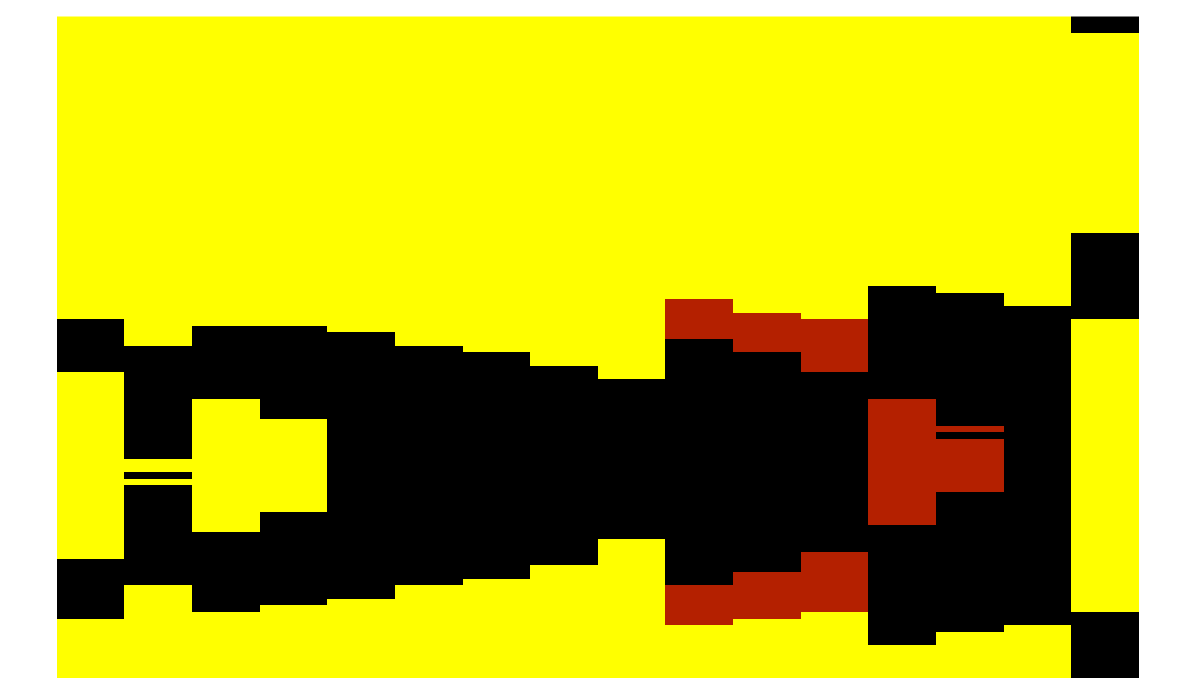
\includegraphics[width=3.7in,height=3.11in]{role-naked.png}};
%% generated with GNUPLOT 6.0p4 (Lua 5.4; terminal rev. Jun 2020, script rev. 120)
%% Mon Jul  6 14:24:11 2026
\path (0.000,0.000) rectangle (12.500,8.750);
\gpcolor{color=gp lt color border}
\gpsetlinetype{gp lt border}
\gpsetdashtype{gp dt solid}
\gpsetlinewidth{2.00}
\draw[gp path] (1.320,0.985)--(1.500,0.985);
\node[gp node right] at (1.136,0.985) {$1$};
\draw[gp path] (1.320,2.476)--(1.500,2.476);
\node[gp node right] at (1.136,2.476) {$20$};
\draw[gp path] (1.320,3.967)--(1.500,3.967);
\node[gp node right] at (1.136,3.967) {$40$};
\draw[gp path] (1.320,5.459)--(1.500,5.459);
\node[gp node right] at (1.136,5.459) {$60$};
\draw[gp path] (1.320,6.950)--(1.500,6.950);
\node[gp node right] at (1.136,6.950) {$80$};
\draw[gp path] (1.320,8.441)--(1.500,8.441);
\node[gp node right] at (1.136,8.441) {$100$};
\draw[gp path] (1.849,0.985)--(1.849,1.165);
\draw[gp path] (1.849,8.441)--(1.849,8.261);
\node[gp node center] at (1.849,0.677) {$1$};
\draw[gp path] (3.436,0.985)--(3.436,1.165);
\draw[gp path] (3.436,8.441)--(3.436,8.261);
\node[gp node center] at (3.436,0.677) {$4$};
\draw[gp path] (5.023,0.985)--(5.023,1.165);
\draw[gp path] (5.023,8.441)--(5.023,8.261);
\node[gp node center] at (5.023,0.677) {$7$};
\draw[gp path] (6.610,0.985)--(6.610,1.165);
\draw[gp path] (6.610,8.441)--(6.610,8.261);
\node[gp node center] at (6.610,0.677) {$10$};
\draw[gp path] (8.197,0.985)--(8.197,1.165);
\draw[gp path] (8.197,8.441)--(8.197,8.261);
\node[gp node center] at (8.197,0.677) {$13$};
\draw[gp path] (9.784,0.985)--(9.784,1.165);
\draw[gp path] (9.784,8.441)--(9.784,8.261);
\node[gp node center] at (9.784,0.677) {$16$};
\node[gp node center] at (0.8,4.713) {$i$};
\node[gp node center] at (5.816,0.215) {chorus cycle $n$};
\gpfill{rgb color={0.000,0.000,0.000}} (10.538,0.985)--(10.987,0.985)--(10.987,1.044)--(10.538,1.044)--cycle;
\gpfill{rgb color={0.088,0.000,0.049}} (10.538,1.043)--(10.987,1.043)--(10.987,1.102)--(10.538,1.102)--cycle;
\gpfill{rgb color={0.125,0.000,0.098}} (10.538,1.101)--(10.987,1.101)--(10.987,1.160)--(10.538,1.160)--cycle;
\gpfill{rgb color={0.153,0.000,0.147}} (10.538,1.159)--(10.987,1.159)--(10.987,1.219)--(10.538,1.219)--cycle;
\gpfill{rgb color={0.177,0.000,0.195}} (10.538,1.218)--(10.987,1.218)--(10.987,1.277)--(10.538,1.277)--cycle;
\gpfill{rgb color={0.198,0.000,0.243}} (10.538,1.276)--(10.987,1.276)--(10.987,1.335)--(10.538,1.335)--cycle;
\gpfill{rgb color={0.217,0.000,0.290}} (10.538,1.334)--(10.987,1.334)--(10.987,1.393)--(10.538,1.393)--cycle;
\gpfill{rgb color={0.234,0.000,0.337}} (10.538,1.392)--(10.987,1.392)--(10.987,1.452)--(10.538,1.452)--cycle;
\gpfill{rgb color={0.250,0.000,0.383}} (10.538,1.451)--(10.987,1.451)--(10.987,1.510)--(10.538,1.510)--cycle;
\gpfill{rgb color={0.265,0.000,0.428}} (10.538,1.509)--(10.987,1.509)--(10.987,1.568)--(10.538,1.568)--cycle;
\gpfill{rgb color={0.280,0.000,0.471}} (10.538,1.567)--(10.987,1.567)--(10.987,1.626)--(10.538,1.626)--cycle;
\gpfill{rgb color={0.293,0.001,0.514}} (10.538,1.625)--(10.987,1.625)--(10.987,1.685)--(10.538,1.685)--cycle;
\gpfill{rgb color={0.306,0.001,0.556}} (10.538,1.684)--(10.987,1.684)--(10.987,1.743)--(10.538,1.743)--cycle;
\gpfill{rgb color={0.319,0.001,0.596}} (10.538,1.742)--(10.987,1.742)--(10.987,1.801)--(10.538,1.801)--cycle;
\gpfill{rgb color={0.331,0.001,0.634}} (10.538,1.800)--(10.987,1.800)--(10.987,1.859)--(10.538,1.859)--cycle;
\gpfill{rgb color={0.342,0.002,0.672}} (10.538,1.858)--(10.987,1.858)--(10.987,1.918)--(10.538,1.918)--cycle;
\gpfill{rgb color={0.354,0.002,0.707}} (10.538,1.917)--(10.987,1.917)--(10.987,1.976)--(10.538,1.976)--cycle;
\gpfill{rgb color={0.364,0.002,0.741}} (10.538,1.975)--(10.987,1.975)--(10.987,2.034)--(10.538,2.034)--cycle;
\gpfill{rgb color={0.375,0.003,0.773}} (10.538,2.033)--(10.987,2.033)--(10.987,2.092)--(10.538,2.092)--cycle;
\gpfill{rgb color={0.385,0.003,0.803}} (10.538,2.091)--(10.987,2.091)--(10.987,2.151)--(10.538,2.151)--cycle;
\gpfill{rgb color={0.395,0.004,0.831}} (10.538,2.150)--(10.987,2.150)--(10.987,2.209)--(10.538,2.209)--cycle;
\gpfill{rgb color={0.405,0.004,0.858}} (10.538,2.208)--(10.987,2.208)--(10.987,2.267)--(10.538,2.267)--cycle;
\gpfill{rgb color={0.415,0.005,0.882}} (10.538,2.266)--(10.987,2.266)--(10.987,2.325)--(10.538,2.325)--cycle;
\gpfill{rgb color={0.424,0.006,0.904}} (10.538,2.324)--(10.987,2.324)--(10.987,2.384)--(10.538,2.384)--cycle;
\gpfill{rgb color={0.433,0.007,0.924}} (10.538,2.383)--(10.987,2.383)--(10.987,2.442)--(10.538,2.442)--cycle;
\gpfill{rgb color={0.442,0.007,0.942}} (10.538,2.441)--(10.987,2.441)--(10.987,2.500)--(10.538,2.500)--cycle;
\gpfill{rgb color={0.451,0.008,0.957}} (10.538,2.499)--(10.987,2.499)--(10.987,2.558)--(10.538,2.558)--cycle;
\gpfill{rgb color={0.459,0.009,0.970}} (10.538,2.557)--(10.987,2.557)--(10.987,2.617)--(10.538,2.617)--cycle;
\gpfill{rgb color={0.468,0.010,0.981}} (10.538,2.616)--(10.987,2.616)--(10.987,2.675)--(10.538,2.675)--cycle;
\gpfill{rgb color={0.476,0.012,0.989}} (10.538,2.674)--(10.987,2.674)--(10.987,2.733)--(10.538,2.733)--cycle;
\gpfill{rgb color={0.484,0.013,0.995}} (10.538,2.732)--(10.987,2.732)--(10.987,2.791)--(10.538,2.791)--cycle;
\gpfill{rgb color={0.492,0.014,0.999}} (10.538,2.790)--(10.987,2.790)--(10.987,2.850)--(10.538,2.850)--cycle;
\gpfill{rgb color={0.500,0.016,1.000}} (10.538,2.849)--(10.987,2.849)--(10.987,2.908)--(10.538,2.908)--cycle;
\gpfill{rgb color={0.508,0.017,0.999}} (10.538,2.907)--(10.987,2.907)--(10.987,2.966)--(10.538,2.966)--cycle;
\gpfill{rgb color={0.515,0.019,0.995}} (10.538,2.965)--(10.987,2.965)--(10.987,3.024)--(10.538,3.024)--cycle;
\gpfill{rgb color={0.523,0.020,0.989}} (10.538,3.023)--(10.987,3.023)--(10.987,3.083)--(10.538,3.083)--cycle;
\gpfill{rgb color={0.530,0.022,0.981}} (10.538,3.082)--(10.987,3.082)--(10.987,3.141)--(10.538,3.141)--cycle;
\gpfill{rgb color={0.538,0.024,0.970}} (10.538,3.140)--(10.987,3.140)--(10.987,3.199)--(10.538,3.199)--cycle;
\gpfill{rgb color={0.545,0.026,0.957}} (10.538,3.198)--(10.987,3.198)--(10.987,3.257)--(10.538,3.257)--cycle;
\gpfill{rgb color={0.552,0.028,0.942}} (10.538,3.256)--(10.987,3.256)--(10.987,3.316)--(10.538,3.316)--cycle;
\gpfill{rgb color={0.559,0.031,0.924}} (10.538,3.315)--(10.987,3.315)--(10.987,3.374)--(10.538,3.374)--cycle;
\gpfill{rgb color={0.566,0.033,0.904}} (10.538,3.373)--(10.987,3.373)--(10.987,3.432)--(10.538,3.432)--cycle;
\gpfill{rgb color={0.573,0.035,0.882}} (10.538,3.431)--(10.987,3.431)--(10.987,3.490)--(10.538,3.490)--cycle;
\gpfill{rgb color={0.580,0.038,0.858}} (10.538,3.489)--(10.987,3.489)--(10.987,3.549)--(10.538,3.549)--cycle;
\gpfill{rgb color={0.586,0.041,0.831}} (10.538,3.548)--(10.987,3.548)--(10.987,3.607)--(10.538,3.607)--cycle;
\gpfill{rgb color={0.593,0.043,0.803}} (10.538,3.606)--(10.987,3.606)--(10.987,3.665)--(10.538,3.665)--cycle;
\gpfill{rgb color={0.599,0.046,0.773}} (10.538,3.664)--(10.987,3.664)--(10.987,3.723)--(10.538,3.723)--cycle;
\gpfill{rgb color={0.606,0.050,0.741}} (10.538,3.722)--(10.987,3.722)--(10.987,3.782)--(10.538,3.782)--cycle;
\gpfill{rgb color={0.612,0.053,0.707}} (10.538,3.781)--(10.987,3.781)--(10.987,3.840)--(10.538,3.840)--cycle;
\gpfill{rgb color={0.619,0.056,0.672}} (10.538,3.839)--(10.987,3.839)--(10.987,3.898)--(10.538,3.898)--cycle;
\gpfill{rgb color={0.625,0.060,0.634}} (10.538,3.897)--(10.987,3.897)--(10.987,3.956)--(10.538,3.956)--cycle;
\gpfill{rgb color={0.631,0.063,0.596}} (10.538,3.955)--(10.987,3.955)--(10.987,4.015)--(10.538,4.015)--cycle;
\gpfill{rgb color={0.637,0.067,0.556}} (10.538,4.014)--(10.987,4.014)--(10.987,4.073)--(10.538,4.073)--cycle;
\gpfill{rgb color={0.643,0.071,0.514}} (10.538,4.072)--(10.987,4.072)--(10.987,4.131)--(10.538,4.131)--cycle;
\gpfill{rgb color={0.650,0.075,0.471}} (10.538,4.130)--(10.987,4.130)--(10.987,4.189)--(10.538,4.189)--cycle;
\gpfill{rgb color={0.656,0.079,0.428}} (10.538,4.188)--(10.987,4.188)--(10.987,4.248)--(10.538,4.248)--cycle;
\gpfill{rgb color={0.661,0.084,0.383}} (10.538,4.247)--(10.987,4.247)--(10.987,4.306)--(10.538,4.306)--cycle;
\gpfill{rgb color={0.667,0.088,0.337}} (10.538,4.305)--(10.987,4.305)--(10.987,4.364)--(10.538,4.364)--cycle;
\gpfill{rgb color={0.673,0.093,0.290}} (10.538,4.363)--(10.987,4.363)--(10.987,4.422)--(10.538,4.422)--cycle;
\gpfill{rgb color={0.679,0.098,0.243}} (10.538,4.421)--(10.987,4.421)--(10.987,4.481)--(10.538,4.481)--cycle;
\gpfill{rgb color={0.685,0.103,0.195}} (10.538,4.480)--(10.987,4.480)--(10.987,4.539)--(10.538,4.539)--cycle;
\gpfill{rgb color={0.690,0.108,0.147}} (10.538,4.538)--(10.987,4.538)--(10.987,4.597)--(10.538,4.597)--cycle;
\gpfill{rgb color={0.696,0.114,0.098}} (10.538,4.596)--(10.987,4.596)--(10.987,4.655)--(10.538,4.655)--cycle;
\gpfill{rgb color={0.702,0.119,0.049}} (10.538,4.654)--(10.987,4.654)--(10.987,4.714)--(10.538,4.714)--cycle;
\gpfill{rgb color={0.707,0.125,0.000}} (10.538,4.713)--(10.987,4.713)--(10.987,4.772)--(10.538,4.772)--cycle;
\gpfill{rgb color={0.713,0.131,0.000}} (10.538,4.771)--(10.987,4.771)--(10.987,4.830)--(10.538,4.830)--cycle;
\gpfill{rgb color={0.718,0.137,0.000}} (10.538,4.829)--(10.987,4.829)--(10.987,4.888)--(10.538,4.888)--cycle;
\gpfill{rgb color={0.723,0.143,0.000}} (10.538,4.887)--(10.987,4.887)--(10.987,4.947)--(10.538,4.947)--cycle;
\gpfill{rgb color={0.729,0.150,0.000}} (10.538,4.946)--(10.987,4.946)--(10.987,5.005)--(10.538,5.005)--cycle;
\gpfill{rgb color={0.734,0.157,0.000}} (10.538,5.004)--(10.987,5.004)--(10.987,5.063)--(10.538,5.063)--cycle;
\gpfill{rgb color={0.740,0.164,0.000}} (10.538,5.062)--(10.987,5.062)--(10.987,5.121)--(10.538,5.121)--cycle;
\gpfill{rgb color={0.745,0.171,0.000}} (10.538,5.120)--(10.987,5.120)--(10.987,5.180)--(10.538,5.180)--cycle;
\gpfill{rgb color={0.750,0.178,0.000}} (10.538,5.179)--(10.987,5.179)--(10.987,5.238)--(10.538,5.238)--cycle;
\gpfill{rgb color={0.755,0.185,0.000}} (10.538,5.237)--(10.987,5.237)--(10.987,5.296)--(10.538,5.296)--cycle;
\gpfill{rgb color={0.760,0.193,0.000}} (10.538,5.295)--(10.987,5.295)--(10.987,5.354)--(10.538,5.354)--cycle;
\gpfill{rgb color={0.765,0.201,0.000}} (10.538,5.353)--(10.987,5.353)--(10.987,5.413)--(10.538,5.413)--cycle;
\gpfill{rgb color={0.771,0.209,0.000}} (10.538,5.412)--(10.987,5.412)--(10.987,5.471)--(10.538,5.471)--cycle;
\gpfill{rgb color={0.776,0.218,0.000}} (10.538,5.470)--(10.987,5.470)--(10.987,5.529)--(10.538,5.529)--cycle;
\gpfill{rgb color={0.781,0.226,0.000}} (10.538,5.528)--(10.987,5.528)--(10.987,5.587)--(10.538,5.587)--cycle;
\gpfill{rgb color={0.786,0.235,0.000}} (10.538,5.586)--(10.987,5.586)--(10.987,5.646)--(10.538,5.646)--cycle;
\gpfill{rgb color={0.791,0.244,0.000}} (10.538,5.645)--(10.987,5.645)--(10.987,5.704)--(10.538,5.704)--cycle;
\gpfill{rgb color={0.795,0.253,0.000}} (10.538,5.703)--(10.987,5.703)--(10.987,5.762)--(10.538,5.762)--cycle;
\gpfill{rgb color={0.800,0.263,0.000}} (10.538,5.761)--(10.987,5.761)--(10.987,5.820)--(10.538,5.820)--cycle;
\gpfill{rgb color={0.805,0.273,0.000}} (10.538,5.819)--(10.987,5.819)--(10.987,5.879)--(10.538,5.879)--cycle;
\gpfill{rgb color={0.810,0.283,0.000}} (10.538,5.878)--(10.987,5.878)--(10.987,5.937)--(10.538,5.937)--cycle;
\gpfill{rgb color={0.815,0.293,0.000}} (10.538,5.936)--(10.987,5.936)--(10.987,5.995)--(10.538,5.995)--cycle;
\gpfill{rgb color={0.820,0.303,0.000}} (10.538,5.994)--(10.987,5.994)--(10.987,6.053)--(10.538,6.053)--cycle;
\gpfill{rgb color={0.824,0.314,0.000}} (10.538,6.052)--(10.987,6.052)--(10.987,6.112)--(10.538,6.112)--cycle;
\gpfill{rgb color={0.829,0.325,0.000}} (10.538,6.111)--(10.987,6.111)--(10.987,6.170)--(10.538,6.170)--cycle;
\gpfill{rgb color={0.834,0.336,0.000}} (10.538,6.169)--(10.987,6.169)--(10.987,6.228)--(10.538,6.228)--cycle;
\gpfill{rgb color={0.839,0.348,0.000}} (10.538,6.227)--(10.987,6.227)--(10.987,6.286)--(10.538,6.286)--cycle;
\gpfill{rgb color={0.843,0.359,0.000}} (10.538,6.285)--(10.987,6.285)--(10.987,6.345)--(10.538,6.345)--cycle;
\gpfill{rgb color={0.848,0.371,0.000}} (10.538,6.344)--(10.987,6.344)--(10.987,6.403)--(10.538,6.403)--cycle;
\gpfill{rgb color={0.852,0.384,0.000}} (10.538,6.402)--(10.987,6.402)--(10.987,6.461)--(10.538,6.461)--cycle;
\gpfill{rgb color={0.857,0.396,0.000}} (10.538,6.460)--(10.987,6.460)--(10.987,6.519)--(10.538,6.519)--cycle;
\gpfill{rgb color={0.862,0.409,0.000}} (10.538,6.518)--(10.987,6.518)--(10.987,6.578)--(10.538,6.578)--cycle;
\gpfill{rgb color={0.866,0.422,0.000}} (10.538,6.577)--(10.987,6.577)--(10.987,6.636)--(10.538,6.636)--cycle;
\gpfill{rgb color={0.871,0.435,0.000}} (10.538,6.635)--(10.987,6.635)--(10.987,6.694)--(10.538,6.694)--cycle;
\gpfill{rgb color={0.875,0.449,0.000}} (10.538,6.693)--(10.987,6.693)--(10.987,6.752)--(10.538,6.752)--cycle;
\gpfill{rgb color={0.879,0.463,0.000}} (10.538,6.751)--(10.987,6.751)--(10.987,6.811)--(10.538,6.811)--cycle;
\gpfill{rgb color={0.884,0.477,0.000}} (10.538,6.810)--(10.987,6.810)--(10.987,6.869)--(10.538,6.869)--cycle;
\gpfill{rgb color={0.888,0.491,0.000}} (10.538,6.868)--(10.987,6.868)--(10.987,6.927)--(10.538,6.927)--cycle;
\gpfill{rgb color={0.893,0.506,0.000}} (10.538,6.926)--(10.987,6.926)--(10.987,6.985)--(10.538,6.985)--cycle;
\gpfill{rgb color={0.897,0.521,0.000}} (10.538,6.984)--(10.987,6.984)--(10.987,7.044)--(10.538,7.044)--cycle;
\gpfill{rgb color={0.901,0.536,0.000}} (10.538,7.043)--(10.987,7.043)--(10.987,7.102)--(10.538,7.102)--cycle;
\gpfill{rgb color={0.906,0.552,0.000}} (10.538,7.101)--(10.987,7.101)--(10.987,7.160)--(10.538,7.160)--cycle;
\gpfill{rgb color={0.910,0.568,0.000}} (10.538,7.159)--(10.987,7.159)--(10.987,7.218)--(10.538,7.218)--cycle;
\gpfill{rgb color={0.914,0.584,0.000}} (10.538,7.217)--(10.987,7.217)--(10.987,7.277)--(10.538,7.277)--cycle;
\gpfill{rgb color={0.919,0.601,0.000}} (10.538,7.276)--(10.987,7.276)--(10.987,7.335)--(10.538,7.335)--cycle;
\gpfill{rgb color={0.923,0.618,0.000}} (10.538,7.334)--(10.987,7.334)--(10.987,7.393)--(10.538,7.393)--cycle;
\gpfill{rgb color={0.927,0.635,0.000}} (10.538,7.392)--(10.987,7.392)--(10.987,7.451)--(10.538,7.451)--cycle;
\gpfill{rgb color={0.931,0.652,0.000}} (10.538,7.450)--(10.987,7.450)--(10.987,7.510)--(10.538,7.510)--cycle;
\gpfill{rgb color={0.935,0.670,0.000}} (10.538,7.509)--(10.987,7.509)--(10.987,7.568)--(10.538,7.568)--cycle;
\gpfill{rgb color={0.940,0.688,0.000}} (10.538,7.567)--(10.987,7.567)--(10.987,7.626)--(10.538,7.626)--cycle;
\gpfill{rgb color={0.944,0.706,0.000}} (10.538,7.625)--(10.987,7.625)--(10.987,7.684)--(10.538,7.684)--cycle;
\gpfill{rgb color={0.948,0.725,0.000}} (10.538,7.683)--(10.987,7.683)--(10.987,7.743)--(10.538,7.743)--cycle;
\gpfill{rgb color={0.952,0.744,0.000}} (10.538,7.742)--(10.987,7.742)--(10.987,7.801)--(10.538,7.801)--cycle;
\gpfill{rgb color={0.956,0.764,0.000}} (10.538,7.800)--(10.987,7.800)--(10.987,7.859)--(10.538,7.859)--cycle;
\gpfill{rgb color={0.960,0.783,0.000}} (10.538,7.858)--(10.987,7.858)--(10.987,7.917)--(10.538,7.917)--cycle;
\gpfill{rgb color={0.964,0.804,0.000}} (10.538,7.916)--(10.987,7.916)--(10.987,7.976)--(10.538,7.976)--cycle;
\gpfill{rgb color={0.968,0.824,0.000}} (10.538,7.975)--(10.987,7.975)--(10.987,8.034)--(10.538,8.034)--cycle;
\gpfill{rgb color={0.972,0.845,0.000}} (10.538,8.033)--(10.987,8.033)--(10.987,8.092)--(10.538,8.092)--cycle;
\gpfill{rgb color={0.976,0.866,0.000}} (10.538,8.091)--(10.987,8.091)--(10.987,8.150)--(10.538,8.150)--cycle;
\gpfill{rgb color={0.980,0.887,0.000}} (10.538,8.149)--(10.987,8.149)--(10.987,8.209)--(10.538,8.209)--cycle;
\gpfill{rgb color={0.984,0.909,0.000}} (10.538,8.208)--(10.987,8.208)--(10.987,8.267)--(10.538,8.267)--cycle;
\gpfill{rgb color={0.988,0.931,0.000}} (10.538,8.266)--(10.987,8.266)--(10.987,8.325)--(10.538,8.325)--cycle;
\gpfill{rgb color={0.992,0.954,0.000}} (10.538,8.324)--(10.987,8.324)--(10.987,8.383)--(10.538,8.383)--cycle;
\gpfill{rgb color={0.996,0.977,0.000}} (10.538,8.382)--(10.987,8.382)--(10.987,8.441)--(10.538,8.441)--cycle;
\draw[gp path] (10.538,0.985)--(10.987,0.985)--(10.987,8.441)--(10.538,8.441)--cycle;
\draw[gp path] (10.987,0.985)--(10.807,0.985);
\node[gp node left] at (11.171,0.985) {$0$};
\draw[gp path] (10.538,0.985)--(10.718,0.985);
\draw[gp path] (10.987,2.476)--(10.807,2.476);
\node[gp node left] at (11.171,2.476) {$0.2$};
\draw[gp path] (10.538,2.476)--(10.718,2.476);
\draw[gp path] (10.987,3.967)--(10.807,3.967);
\node[gp node left] at (11.171,3.967) {$0.4$};
\draw[gp path] (10.538,3.967)--(10.718,3.967);
\draw[gp path] (10.987,5.458)--(10.807,5.458);
\node[gp node left] at (11.171,5.458) {$0.6$};
\draw[gp path] (10.538,5.458)--(10.718,5.458);
\draw[gp path] (10.987,6.949)--(10.807,6.949);
\node[gp node left] at (11.171,6.949) {$0.8$};
\draw[gp path] (10.538,6.949)--(10.718,6.949);
\draw[gp path] (10.987,8.441)--(10.807,8.441);
\node[gp node left] at (11.171,8.441) {$1$};
\draw[gp path] (10.538,8.441)--(10.718,8.441);
\node[gp node center] at (10.8,.215) {$R_i^{(n)}$};
%% coordinates of the plot area
\gpdefrectangularnode{gp plot 1}{\pgfpoint{1.320cm}{0.985cm}}{\pgfpoint{10.313cm}{8.441cm}}
\end{tikzpicture}
%% gnuplot variables
\end{document}
